\section{Results}
\label{sec:results}

\subsection{Baseline Performance}
\label{sec:baselines}

\Tabref{tab:baselines} shows the zero-shot accuracy of \qwen across all benchmarks. The model performs best on \arc (0.800) and worst on \gsmk (0.160), establishing a wide dynamic range for measuring fine-tuning effects.

\begin{table}[t]
\centering
\caption{Baseline (zero-shot) accuracy of \qwen on each benchmark. Random chance is shown for reference. \gsmk and \gsmsym have near-identical baselines, confirming they test the same capability.}
\label{tab:baselines}
\vspace{4pt}
\begin{tabular}{@{}lccr@{}}
\toprule
\textsc{Benchmark} & \textsc{Accuracy} & \textsc{Chance} & \textsc{Correct / Total} \\
\midrule
\arc        & 0.800 & 0.25 & 400 / 500 \\
\mmlu       & 0.610 & 0.25 & 305 / 500 \\
\wino       & 0.573 & 0.50 & 172 / 300 \\
\mmlupro    & 0.344 & 0.10 & 172 / 500 \\
\gpqa       & 0.308 & 0.25 & 138 / 448 \\
\gsmsym     & 0.167 & $\sim$0 & 50 / 300 \\
\gsmk       & 0.160 & $\sim$0 & 48 / 300 \\
\bottomrule
\end{tabular}
\end{table}

\subsection{Cross-Benchmark Fine-tuning Results}
\label{sec:cross}

\Tabref{tab:heatmap} presents the accuracy change after fine-tuning, evaluated across all benchmarks. Each row represents a different fine-tuning condition; each column is an evaluation benchmark. Bold values on the diagonal indicate self-evaluation (same benchmark as training data).

\begin{table}[t]
\centering
\caption{Accuracy change ($\Delta$) after fine-tuning on each benchmark's training data, evaluated across all benchmarks. Bold diagonal entries are self-evaluations. \increase and \decrease indicate the direction of change. Fine-tuning on any benchmark dramatically improves \gsmk and \gsmsym.}
\label{tab:heatmap}
\vspace{4pt}
\resizebox{\textwidth}{!}{%
\begin{tabular}{@{}lccccccc@{}}
\toprule
& \multicolumn{2}{c}{\textsc{Math}} & \multicolumn{2}{c}{\textsc{Knowledge}} & \textsc{Commonsense} & \textsc{Science} & \textsc{Expert} \\
\cmidrule(lr){2-3} \cmidrule(lr){4-5} \cmidrule(lr){6-6} \cmidrule(lr){7-7} \cmidrule(lr){8-8}
\textsc{FT Dataset} & \textsc{GSM8K} & \textsc{GSM-Sym} & \textsc{MMLU} & \textsc{MMLU-Pro} & \textsc{WinoGr.} & \textsc{ARC} & \textsc{GPQA} \\
\midrule
\gsmk   & {\bf +.557}\increase & +.370\increase & +.014 & +.008 & +.023 & $-.014$ & +.011 \\
\mmlu   & +.360\increase & +.233\increase & {\bf +.016} & +.022 & +.007 & $-.014$ & $-.009$ \\
\wino   & +.163\increase & +.087\increase & $-.032$\decrease & $-.012$ & {\bf +.137}\increase & $-.024$ & +.004 \\
\arc    & +.357\increase & +.327\increase & +.034 & $-.020$ & +.017 & {\bf +.030} & +.002 \\
\bottomrule
\end{tabular}}
\end{table}

\begin{figure}[t]
\centering
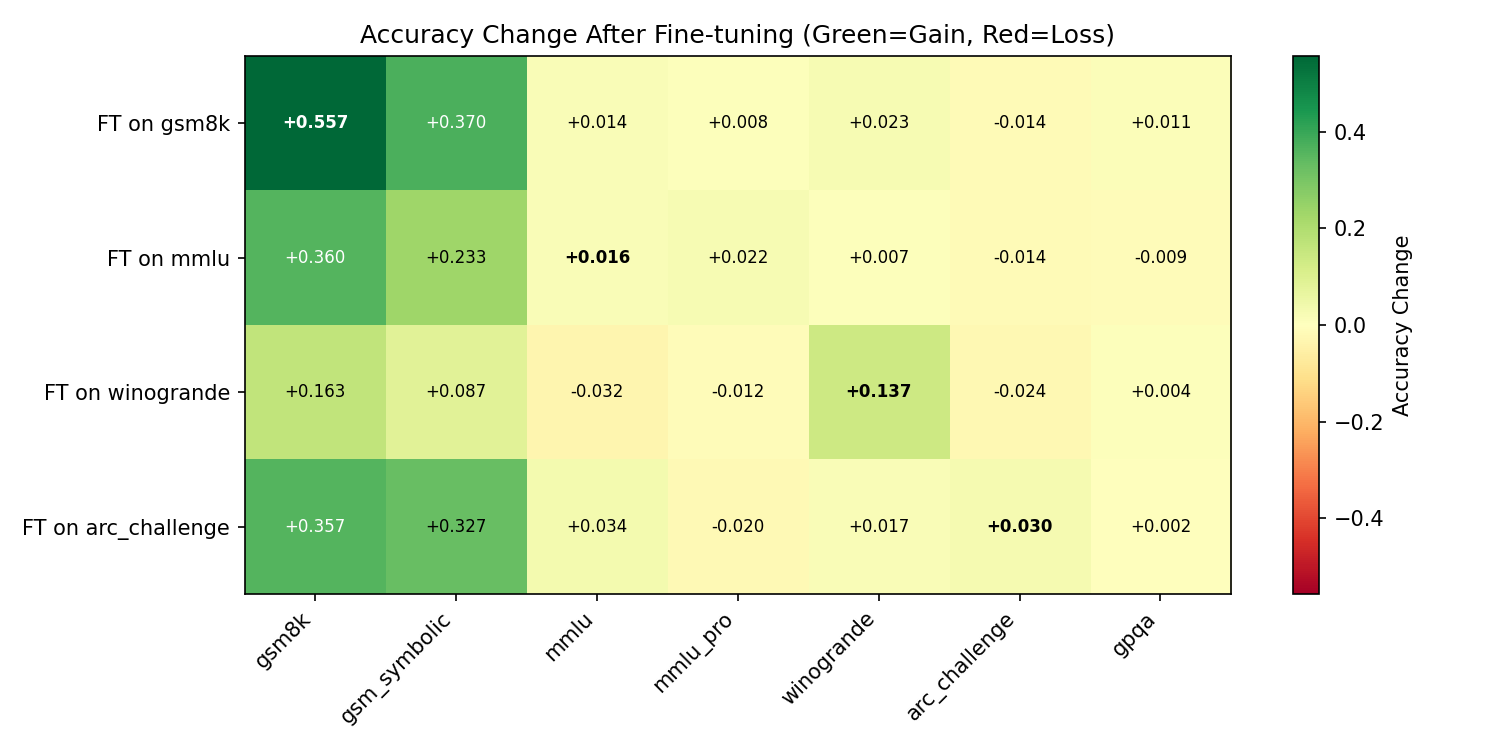
\includegraphics[width=0.95\linewidth]{figures/finetuning_gains_heatmap.png}
\caption{Heatmap of accuracy changes after fine-tuning. Rows are fine-tuning conditions; columns are evaluation benchmarks. The \gsmk and \gsmsym columns are consistently warm across all conditions, indicating these benchmarks are improved by general instruction tuning. \gpqa and \mmlupro columns remain cool, reflecting their resistance.}
\label{fig:heatmap}
\end{figure}

Three patterns emerge from the heatmap. First, the \gsmk and \gsmsym columns show large positive gains under every fine-tuning condition---even when the training data has no mathematical content (\eg \wino commonsense problems yield +0.163 on \gsmk). Second, the \gpqa column is near zero across all conditions (maximum +0.011), confirming its resistance. Third, the \mmlupro column averages $-0.001$ across conditions, showing effective immunity.

\subsection{Finetuning Resistance Ranking}
\label{sec:ranking}

\Tabref{tab:resistance} presents our main result: a ranking of benchmarks by finetuning resistance. We compute the resistance score from \eqref{eq:resistance} for benchmarks with training data, and report the maximum observed gain for evaluation-only benchmarks.

\begin{table}[t]
\centering
\caption{Finetuning resistance ranking. Higher resistance scores indicate greater robustness to memorization-driven inflation. \gpqa and \mmlupro are effectively immune. \wino is the least resistant despite its bias-reduction design.}
\label{tab:resistance}
\vspace{4pt}
\begin{tabular}{@{}clcccc@{}}
\toprule
\textsc{Rank} & \textsc{Benchmark} & \textsc{Resistance} & \textsc{Self Gain} & \textsc{Inflation} & \textsc{Category} \\
\midrule
1 & \gpqa       & $\sim$1.0 & N/A    & max +.011  & Expert knowledge \\
2 & \mmlupro    & $\sim$1.0 & N/A    & avg $-.001$ & Harder variant \\
3 & \mmlu       & {\bf 1.000}  & +.016  & $-.006$    & Large, diverse \\
4 & \arc        & {\bf 1.000}  & +.030  & $-.089$    & Science reasoning \\
5 & \gsmk       & 0.665     & +.557  & +.187      & Template math \\
6 & \wino       & 0.227     & +.137  & +.106      & Binary commonsense \\
\bottomrule
\end{tabular}
\end{table}

\begin{figure}[t]
\centering
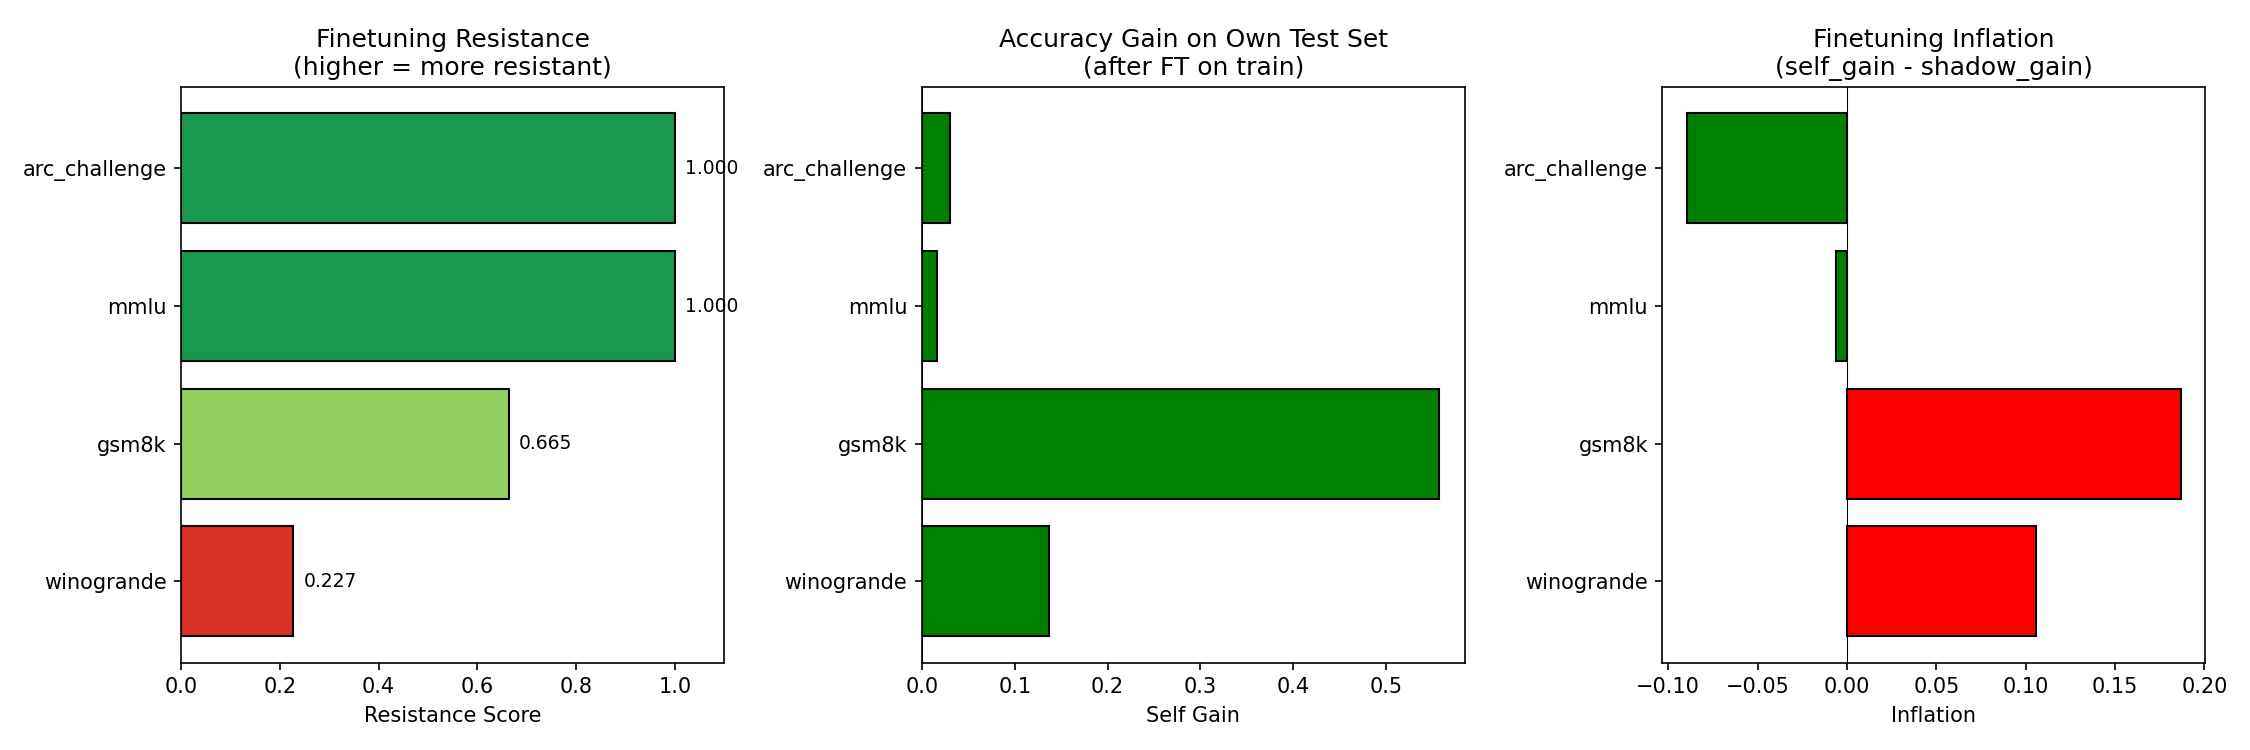
\includegraphics[width=0.85\linewidth]{figures/resistance_ranking.png}
\caption{Finetuning resistance scores across benchmarks. Expert-knowledge benchmarks (\gpqa) and harder variants (\mmlupro) achieve near-perfect resistance. \wino's AFLITE bias reduction does not prevent finetuning inflation.}
\label{fig:resistance}
\end{figure}

\subsection{Shadow Benchmark Analysis}
\label{sec:shadow}

The \gsmk--\gsmsym pair provides the cleanest test of finetuning inflation. Fine-tuning on \gsmk improves \gsmk accuracy by +0.557 but only improves \gsmsym by +0.370---a gap of 0.187 (34\% inflation). Both gains are individually significant ($p < 0.0001$), confirming this is a reliable measurement. The inflation gap means that roughly one-third of \gsmk's fine-tuning improvement reflects memorization of specific instances rather than genuine mathematical capability.

For the \mmlu--\mmlupro pair, fine-tuning on \mmlu actually improves \mmlupro more (+0.022) than \mmlu itself (+0.016), yielding \emph{negative} inflation. However, neither gain is statistically significant ($p = 0.60$ for \mmlu's self-gain), so we interpret this as \mmlu being effectively immune to fine-tuning at this scale---the training data is too large and diverse for \lora with 3{,}000 samples to produce measurable memorization.

\subsection{Statistical Significance}
\label{sec:stats}

We assess significance using McNemar's test for paired proportions (\tabref{tab:significance}).

\begin{table}[t]
\centering
\caption{Statistical significance of key results. Only \gsmk, \gsmsym, and \wino show significant fine-tuning effects. \mmlu, \arc, and \gpqa gains are not significant.}
\label{tab:significance}
\vspace{4pt}
\begin{tabular}{@{}llcc@{}}
\toprule
\textsc{Comparison} & \textsc{$\Delta$ Accuracy} & \textsc{$p$-value} & \textsc{Significant?} \\
\midrule
\gsmk self-gain (FT on \gsmk)      & +0.557 & $<$0.0001 & Yes \\
\gsmsym gain (FT on \gsmk)          & +0.370 & $<$0.0001 & Yes \\
\wino self-gain (FT on \wino)       & +0.137 & 0.0005    & Yes \\
\gsmk gain (FT on \mmlu)            & +0.360 & $<$0.0001 & Yes \\
\gsmk gain (FT on \arc)             & +0.357 & $<$0.0001 & Yes \\
\gsmk gain (FT on \wino)            & +0.163 & $<$0.0001 & Yes \\
\mmlu self-gain (FT on \mmlu)       & +0.016 & 0.60      & No \\
\arc self-gain (FT on \arc)         & +0.030 & 0.22      & No \\
\gpqa change (any FT)               & $\leq$+0.011 & $>$0.70   & No \\
\bottomrule
\end{tabular}
\end{table}

\subsection{Hypothesis Testing}
\label{sec:hypotheses}

We evaluate four pre-registered hypotheses:

\para{H1: \gsmsym resists \gsmk fine-tuning.} \emph{Partially supported.} \gsmsym gained +0.370 versus \gsmk's +0.557, showing meaningful resistance (66.5\% of gain is genuine) but not immunity. Template randomization reduces but does not eliminate memorization.

\para{H2: Harder benchmarks are more resistant.} \emph{Supported.} \gpqa (hardest) and \mmlupro (harder \mmlu) showed near-zero gains under all conditions. Difficulty is strongly correlated with resistance.

\para{H3: Bias-reduced \wino is moderately resistant.} \emph{Refuted.} \wino was the \emph{least} resistant benchmark (score 0.227). AFLITE removes statistical shortcuts from the static dataset but does not prevent fine-tuning from learning task-specific binary patterns.

\para{H4: No benchmark is fully finetuning-proof.} \emph{Partially supported.} \gpqa and \mmlupro appear effectively proof in our experiments, though we note the caveat that \gpqa was not directly fine-tuned on (no training split available) and \mmlupro's resistance may partly reflect our model's limited capacity.
